\chapter{立体视觉与三角测量的光学限度}
\label{ch:07}

\section{效果}
\label{sec:ch07-effect}

读完本章，你应能：
\begin{enumerate}
  \item 由基线 $B$、焦距 $f_x$ 与视差写出三角测量关系，并推导误差放大 $\delta Z\sim Z^2\delta d/(Bf_x)$；
  \item 说明交会角如何同时影响精度、遮挡与匹配难度；
  \item 解释景深与基线之间的冲突，以及它为何常常决定紧凑探头的上限；
  \item 把标定误差（内参、外参、畸变）沿三角测量传播到 $(X,Y,Z)$；
  \item 比较相机–投影仪对与双相机立体，并为口内扫描仪做一份精度预算。
\end{enumerate}

\section{原理}
\label{sec:ch07-principle}

\subsection{投影与三角测量}

沿用第~\ref{ch:02}~章的针孔模型：
\begin{equation}
  s\begin{pmatrix}u\\v\\1\end{pmatrix}=K\,[R\mid t]\begin{pmatrix}X\\Y\\Z\\1\end{pmatrix},
  \label{eq:ch07-proj}
\end{equation}
$s$ 为齐次尺度。两个视图（两台相机，或相机与投影仪）各给出一条射线，射线的交点即为物点。实际中两射线因噪声不相交，常取最小化重投影误差的点 \citep{HartleyZisserman2004}。

\textbf{平行校正的标准形。} 两个相机光轴平行、基线 $B$ 沿 $X$ 方向、焦距同为 $f_x$（像素单位，$f_x=f/p$，$f$ 为毫米焦距、$p$ 为像元间距）。视差 $d=u_1-u_2$，则
\begin{equation}
  Z=\frac{Bf_x}{d}.
  \label{eq:ch07-disparity}
\end{equation}
对 $d$ 求导：
\begin{equation}
  \delta Z=\frac{Bf_x}{d^2}\,\delta d=\frac{Z^2}{Bf_x}\,\delta d.
  \label{eq:ch07-error}
\end{equation}
这就是第~\ref{ch:02}~章预告的误差放大。记号约定：$\delta u$ 表示单个视图中的像面定位误差，$\delta d$ 表示视差误差。双相机且两侧误差独立同分布时 $\delta d=\sqrt2\,\delta u$；相机–投影仪对中投影侧坐标由相位给出，$\delta d$ 即相位误差折算到相机像素的等效值。第~\ref{ch:02}~章的 $\delta u$ 估计在这里应理解为 $\delta d$ 的来源。三个结论：深度误差随 $Z^2$ 增长；与基线、焦距成反比；与匹配精度 $\delta d$（亚像素级）成正比（图~\ref{fig:ch07-tri}）。

对结构光，$\delta d$ 来自第~\ref{ch:06}~章的相位噪声：$\delta u_p=\dfrac{P}{2\pi}\sigma_\varphi$，再按投影仪与相机的焦距之比折算。于是「条纹周期 $P$ 越短、调制度越高、$\SNR$ 越高」直接转化为更小的 $\delta Z$。

\textbf{横向误差。} $X=Zu'/f_x$（$u'$ 为相对主点的坐标），故 $\delta X\approx (Z/f_x)\delta u+(X/Z)\delta Z$。横向误差主要随 $Z$ 线性增长，通常小于深度误差，除非视场边缘 $X/Z$ 较大。

\begin{figure}[htbp]
  \centering
  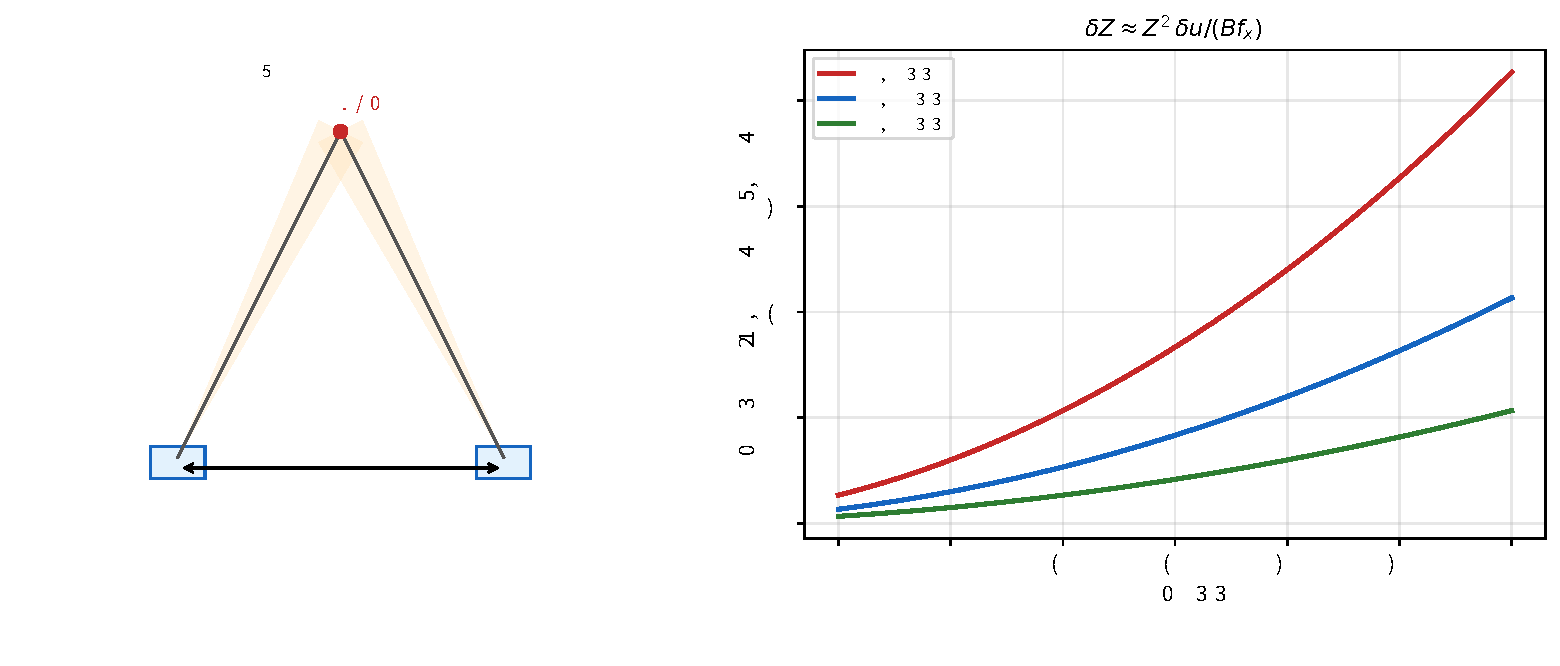
\includegraphics[width=0.98\textwidth]{fig-stereo-triangulation.pdf}
  \caption{三角测量、交会角与误差随工作距和基线变化的概念草图（非精确工程图）。}
  \label{fig:ch07-tri}
\end{figure}

\subsection{匹配精度从哪里来}

式~\eqref{eq:ch07-error} 中的 $\delta d$ 不是一个固定常数，而是光学与信号处理共同决定的量。对被动立体，$\delta d$ 取决于局部纹理的对比度与 $\SNR$：纹理越弱、模糊越重，相关峰越宽，亚像素定位越差。对结构光，$\delta d$ 取决于相位噪声与条纹周期：周期 $P$ 越短，相位误差折算成的像素误差越小，但周期不能短于光学系统在整个景深内能够传递的空间频率，否则调制度 $M$ 先崩溃（第~\ref{ch:03}~章的 $\MTF$ 讨论）。因此，「提高精度」的三条路径——增大基线、增大焦距、降低匹配误差——各自都撞上一个光学墙：基线撞上体积与遮挡，焦距撞上视场与景深，匹配误差撞上 $\MTF$ 与光子噪声。

还应区分相机像素与投影仪像素。投影仪分辨率往往低于相机，但相位编码是连续量，投影仪像素的离散性只在二值或伽马失真时显现；真正限制精度的通常是相机一侧的 $\SNR$ 与模糊。若投影侧离焦严重，条纹在物面已被抹平，相机再清晰也无济于事。设计时可以把两侧的 $\PSF$ 投影到物面上比较，较宽的一侧就是匹配精度的瓶颈。

\subsection{交会角}

非平行配置下，用交会角 $\theta$（两射线在物点的夹角）更直观。若每条射线的角度误差为 $\delta\alpha\approx\delta u/f_x$，则沿二者平分线方向的深度误差约为
\begin{equation}
  \delta Z\approx\frac{Z\,\delta\alpha}{2\sin(\theta/2)},
  \label{eq:ch07-angle}
\end{equation}
小角度时 $2\sin(\theta/2)\approx\theta\approx B/Z$，回到式~\eqref{eq:ch07-error}（两视图噪声独立时再乘约 $\sqrt2$ 的常数因子）。交会角越大，精度越好；但同时：
\begin{itemize}
  \item 两视图看到的表面外观差异更大（透视变形、镜面反射位置不同），匹配更难；
  \item 遮挡与阴影增多；
  \item 对结构光，投影条纹在斜面上压缩或拉伸更明显。
\end{itemize}
经验上交会角常取 $10^\circ$--$30^\circ$，具体取决于场景几何。

\subsection{遮挡与阴影}

三角测量要求物点同时被两个视图看见。双相机系统中，一台相机能看到、另一台看不到的区域称为\textbf{遮挡}。相机–投影仪系统中，投影仪照不到的区域称为\textbf{阴影}，相机看不到的区域同样是遮挡。两者都会导致缺失数据，并且基线越大、表面越陡（牙间隙、龈沟、深窝洞）越严重。

处理方式：多视角拼接（手持扫描不断换角度）；多投影器或多相机；接受部分缺失，由后续融合补洞。其中「缺失」是可诊断的；更危险的是边界处的\textbf{混合像素}：一个像素同时包含前景与背景，或在阴影边缘接收了部分条纹，产生「飞点」。

\subsection{景深与基线的冲突}

精度希望 $B$ 大、$f_x$ 大、$Z$ 小。但：
\begin{itemize}
  \item 景深 $Z_d$ 随相对孔径减小而增大，随焦距增大、工作距减小而迅速缩小（第~\ref{ch:01}~章）。$f_x$ 大且 $Z$ 小意味着景深浅。
  \item 基线 $B$ 大意味着交会角大，同一深度范围内物点在两视图中横移更多，所需的共同视场与有效景深范围被压缩。
  \item 为扩展景深而缩小孔径，会降低通光量与衍射极限分辨（第~\ref{ch:03}~章、第~\ref{ch:05}~章），使 $\delta u$ 变大。
\end{itemize}
因此存在一个最优区间：在给定探头尺寸、工作距与深度范围下，$B$ 与孔径被同时约束。紧凑探头（如口内）往往不是被三角公式限制，而是被「探头头部放不下更大的基线」与「景深要覆盖整颗牙」两条硬约束限制。

\subsection{标定误差传播}

三角测量的输入除了 $(u,v)$ 外，还有 $K$、畸变、$R$、$t$。常见误差：
\begin{itemize}
  \item \textbf{基线长度误差} $\delta B$：由式~\eqref{eq:ch07-disparity}，$\delta Z/Z=\delta B/B$，产生整体尺度误差；对比测量长度（如牙弓跨度）时出现等比例偏差。
  \item \textbf{焦距误差} $\delta f_x$：同样是尺度误差 $\delta Z/Z=\delta f_x/f_x$。
  \item \textbf{主点 / 旋转误差}：等价于视差上的常数偏置 $\Delta d$，$\delta Z\approx Z^2\Delta d/(Bf_x)$，随深度非线性变化，把平面扭成曲面。
  \item \textbf{残余畸变}：在视场边缘产生空间相关的深度误差，常表现为平面重建成「碗形」或「马鞍形」。
\end{itemize}
标定本身使用 \citet{Zhang2000Calibration} 一类方法，其精度受标定板制造误差、角点检测精度、姿态多样性限制。关键原则：标定的深度范围与姿态应覆盖工作范围，否则外推误差会以 $Z^2$ 方式出现。

\subsection{相机–投影仪对与双相机立体}

\begin{itemize}
  \item \textbf{双相机立体}：被动或主动照明。被动立体依赖表面纹理，在光滑釉质上难以匹配；加上随机散斑投影可提供纹理，但不必标定投影仪。对应是二维搜索（沿极线一维）。
  \item \textbf{相机–投影仪对}：对应由相位直接给出，几乎没有匹配歧义；但需要标定投影仪，且投影仪的畸变、伽马、热漂移都进入误差。
  \item \textbf{双相机 + 投影条纹}：用相位作为「纹理」在两相机间匹配，投影仪不进入几何模型，只需相位稳定。代价是两个相机都要看到、多一台相机的体积与成本，以及阴影与遮挡的并集。
\end{itemize}
选型时考虑：哪个器件的几何最稳定（相机通常比投影仪稳定）；体积；遮挡模式；匹配歧义。

\subsection{推导：深度误差的一阶与二阶项}

由相似三角形，平行双目中 $Z=f_xB/d$（式~\eqref{eq:ch07-disparity}）。对 $d$ 求导：
\[
  \frac{\partial Z}{\partial d}=-\frac{f_xB}{d^2}=-\frac{Z^2}{f_xB},
\]
取绝对值即一阶误差 $\delta Z=Z^2\delta d/(f_xB)$。适用条件：$\delta d\ll d$。

\textbf{二阶偏置。} $Z$ 是 $d$ 的凸函数，零均值的视差噪声会让 $Z$ 的期望偏大。设 $d$ 的噪声 $e$ 均值零、方差 $\sigma_d^2$，展开
\[
  \frac{1}{d+e}=\frac1d\Bigl(1-\frac ed+\frac{e^2}{d^2}-\cdots\Bigr),\qquad
  \mathbb E[Z]\approx Z\Bigl(1+\frac{\sigma_d^2}{d^2}\Bigr).
\]
偏置 $Z\sigma_d^2/d^2$。第~\ref{ch:00}~章的几何中 $f_xB=12000\,\mathrm{mm}\cdot$像素、$Z=15\,\mathrm{mm}$，$d=800$ 像素；$\sigma_d=0.051$ 像素时偏置约 $15\times(6\times10^{-5})^2\,\mathrm{mm}$，完全可忽略。但远距被动立体常见 $d\approx20$ 像素、$\sigma_d\approx1$ 像素，偏置为 $Z$ 的 $0.25\%$，在 $Z=4\,\mathrm{m}$ 时约 $1\,\mathrm{cm}$，且平均多帧也不会消失。这提醒我们：对深度取平均之前，最好先对视差取平均。

\subsection{推导：相机射线与投影光平面求交}

结构光常用「相机 + 投影仪」而非两台相机。相位确定投影仪的一列，即空间中一张光平面 $\boldsymbol n^\top\boldsymbol X=h$（在相机坐标系中表示，$\boldsymbol n$ 与 $h$ 由标定给出）。相机像素的归一化射线 $\boldsymbol X=t\,\tilde{\boldsymbol x}$，$\tilde{\boldsymbol x}=(x,y,1)^\top$。代入平面方程：
\[
  t=\frac{h}{\boldsymbol n^\top\tilde{\boldsymbol x}},\qquad Z=t .
\]
每像素只需一次点积与一次除法，适合 GPU 逐像素计算。条件性：当 $\boldsymbol n^\top\tilde{\boldsymbol x}\to0$，射线几乎平行于光平面，$Z$ 对相位与标定误差极端敏感——这正是交会角过小的情形。对平面法向的小误差 $\delta\boldsymbol n$，
\[
  \frac{\delta Z}{Z}\approx-\frac{\delta\boldsymbol n^\top\tilde{\boldsymbol x}}{\boldsymbol n^\top\tilde{\boldsymbol x}},
\]
分母越小，放大越大。实现中应对 $|\boldsymbol n^\top\tilde{\boldsymbol x}|$ 设下限，低于下限的像素直接标为无效，而不是输出一个巨大的深度。

\subsection{例：一张完整的深度误差预算}

把前面各章算过的数放到同一几何（第~\ref{ch:00}~章：$Z=15\,\mathrm{mm}$，$f_xB=12000\,\mathrm{mm}\cdot$像素，$P=16$ 像素，四步相移）下。随机项可按平方和合成；系统项单独列出，因为它们在空间上相关，不随平均下降。数量级示意：

\begin{center}
\small
\begin{tabular}{llll}
  \hline
  来源 & 相位或视差 & $\delta Z$ & 性质\\
  \hline
  光子与读出噪声（第~\ref{ch:05}~章） & $0.020\,\mathrm{rad}$ & $0.96\,\mu\mathrm{m}$ & 随机\\
  伽马残余，四步（第~\ref{ch:06}~章） & $0.0066\,\mathrm{rad}$ & $0.3\,\mu\mathrm{m}$ & 系统波纹\\
  自动曝光跳变 $5\%$（第~\ref{ch:05}~章） & $0.05\,\mathrm{rad}$ & $2.4\,\mu\mathrm{m}$ & 系统波纹\\
  焦距标定误差 $0.1\%$（第~\ref{ch:02}~章） & — & $15\,\mu\mathrm{m}$ & 系统尺度\\
  \hline
\end{tabular}
\end{center}

读表：单帧随机噪声只有约 $1\,\mu\mathrm{m}$，但焦距的千分之一误差直接带来 $15\,\mu\mathrm{m}$ 的整体尺度误差，比随机项大一个数量级。若只看点云「平不平滑」，会误以为系统精度在微米级；只有用已知尺寸的标准件检验才看得到尺度误差。这就是为什么第~\ref{ch:10}~章强调把误差分成随机与系统两类分别核查。

\section{限度}
\label{sec:ch07-limits}

\begin{itemize}
  \item 式~\eqref{eq:ch07-error} 是一阶近似，适用于 $\delta d\ll d$；视差很小（远处或基线很短）时误差分布非对称、有偏。
  \item 误差独立假设：实际中相位误差与标定误差往往空间相关，平均多帧只能降低随机部分。
  \item 针孔模型假设：大视场、显微或远心光学需另行建模（第~\ref{ch:02}~章）。
  \item 本章不讨论多视角融合（ICP、TSDF）的累积误差，那属于系统层面。
\end{itemize}

\section{对象}
\label{sec:ch07-object}

\textbf{口内扫描仪的基线设计。} 典型参数（数量级示意，不对应具体产品）：工作距 $Z\approx15\,\mathrm{mm}$，深度范围约 $\pm5\,\mathrm{mm}$，探头头部宽约 $20\,\mathrm{mm}$，故基线 $B$ 通常在数毫米到十余毫米之间；交会角约 $10^\circ$--$25^\circ$。

\textbf{精度预算。} 设 $f_x=1500$ 像素、$B=8\,\mathrm{mm}$、$Z=15\,\mathrm{mm}$、等效视差误差 $\delta d=0.1$ 像素：
\[
  \delta Z\approx\frac{15^2\times0.1}{8\times1500}\,\mathrm{mm}\approx1.9\,\mu\mathrm{m}.
\]
这是单点、随机噪声部分，看起来远好于临床需要（数十微米）。实际误差主要来自：
\begin{enumerate}
  \item 次表面散射与高反引起的相位偏置（第~\ref{ch:06}~章），可达十余到数十微米，系统性；
  \item 标定残差与温漂：$\delta B/B=10^{-3}$ 即产生 $15\,\mu\mathrm{m}$ 的深度尺度误差；
  \item 景深边缘的调制度下降使 $\delta d$ 增大数倍；
  \item 运动伪影与拼接累积误差（全牙弓尺度上最显著）。
\end{enumerate}
所以口内扫描的单帧精度预算中，三角几何的随机项往往不是瓶颈，模型误差与系统漂移才是。设计时应把预算表写成「随机项 + 每个系统项」，逐项给出量级与诊断方法，而不是只报告 $\delta Z$ 公式值。

\textbf{诊断提示。} 平面板扫描出现碗形：查畸变与主点；不同深度的台阶高度比例偏差：查基线与焦距；仅在湿润或半透明材料上偏差：查散射与高反；随开机时间漂移：查热稳定性与重标定周期。

\section*{本章收束}
三角测量把像面误差以 $Z^2/(Bf_x)$ 放大成深度误差。基线与交会角带来精度，也带来遮挡、匹配难度与景深压力。标定误差中，尺度项、偏置项、畸变项各有特征形状，可以从重建的平面与台阶上诊断出来。口内扫描仪的精度预算主要由系统项而非随机项决定。

\section{习题}
\label{sec:ch07-exercises}

\begin{enumerate}
  \item \textbf{（计算）} $f_x=1200$ 像素、$B=10\,\mathrm{mm}$、$Z=20\,\mathrm{mm}$、$\delta d=0.2$ 像素。求视差 $d$ 与 $\delta Z$。若 $Z$ 增为 $40\,\mathrm{mm}$ 呢？
  \item \textbf{（计算）} 要在 $Z=15\,\mathrm{mm}$ 处达到 $\delta Z\le5\,\mu\mathrm{m}$，$f_x=1500$ 像素、$\delta d=0.15$ 像素，最小基线是多少？
  \item \textbf{（重建场景）} 扫描一个光学平面，点云呈中心低、边缘高的碗形，幅度随视场半径平方增长。最可能是哪项标定误差？
  \item \textbf{（重建场景）} 扫描一组标称 $1.000\,\mathrm{mm}$ 的量块台阶，测得均为 $1.004\,\mathrm{mm}$，且与位置无关。可能原因是什么？如何修正？
  \item \textbf{（重建场景）} 牙间隙中大量缺失点，边界附近有离群飞点。区分阴影、遮挡与混合像素，并分别给出对策。
  \item \textbf{（设计）} 为缩小探头，基线从 $10\,\mathrm{mm}$ 减为 $6\,\mathrm{mm}$。为保持 $\delta Z$，可调哪些量？各自的代价是什么？
  \item \textbf{（比较）} 某团队考虑用「双相机 + 条纹」替代「单相机 + 投影仪」。列出精度、标定、遮挡、体积四个方面的变化。
  \item \textbf{（推导）} 推导二阶偏置 $Z\sigma_d^2/d^2$，并说明为何先平均视差再换算深度能消除它。
  \item \textbf{（计算）} 光平面法向与相机射线夹角为 $80^\circ$（即 $\boldsymbol n^\top\tilde{\boldsymbol x}/|\tilde{\boldsymbol x}|=\cos80^\circ$）。若法向在射线方向的分量误差为 $10^{-3}$，求相对深度误差，并与夹角 $45^\circ$ 时比较。
  \item \textbf{（口扫场景）} 正文预算表中，若伽马残余改用三步（$0.23\,\mathrm{rad}$），预算主导项会变成什么？要让伽马项小于光子噪声项，三步方案需要把伽马残余压到多少（按 $\gamma\approx1.1$ 时 $0.022\,\mathrm{rad}$ 线性插值估计）？
  \item \textbf{（医学重建）} 用于体表的大视场结构光，$Z=500\,\mathrm{mm}$，$f_xB=2.5\times10^5\,\mathrm{mm}\cdot$像素，$\delta d=0.1$ 像素。求一阶 $\delta Z$；若焦距标定误差仍为 $0.1\%$，尺度误差是多少？哪一项主导？
  \item \textbf{（C++/CUDA 实践）} 写出射线—光平面求交的核函数伪代码，包括无效像素判定，并说明 $\boldsymbol n$、$h$ 如何随投影仪列（相位）变化而查表或插值。
\end{enumerate}

\section{习题讲解}
\label{sec:ch07-solutions}

\begin{enumerate}
  \item $d=Bf_x/Z=10\times1200/20=600$ 像素；$\delta Z=Z^2\delta d/(Bf_x)=400\times0.2/12000\approx6.7\,\mu\mathrm{m}$。$Z=40\,\mathrm{mm}$ 时 $d=300$ 像素，$\delta Z\approx26.7\,\mu\mathrm{m}$，为 $4$ 倍。
  \item $B\ge Z^2\delta d/(f_x\delta Z)=225\times0.15/(1500\times0.005)=4.5\,\mathrm{mm}$。
  \item 残余径向畸变（或畸变模型阶数不足）。重新标定、覆盖视场边缘的姿态，检查畸变模型阶数。
  \item 整体尺度误差 $0.4\%$：基线或焦距标定偏差（或标定板尺寸误差）。用已知尺寸的标准件做尺度校正，或重新标定并核对标定板证书。
  \item 阴影：投影仪照不到，相机看得见但无调制，$M$ 低，可用调制度掩膜识别；遮挡：相机看不到，无数据；混合像素：边界像素混合前后景，相位异常，用调制度与相位梯度阈值剔除。对策：多视角拼接、缩小基线、边缘滤波。
  \item 由 $\delta Z\propto Z^2\delta d/(Bf_x)$：增大 $f_x$（视场变小、景深变浅）；减小 $Z$（景深更浅、探头更贴近）；减小 $\delta d$（提高条纹频率与 $\SNR$，或增加帧数，代价是光通量与运动敏感）。
  \item 精度：相位只用作匹配特征，投影仪畸变与伽马不再进入几何，系统性改善；标定：两相机标定更稳定，投影仪无需标定；遮挡：需三者同时可见，缺失增多；体积：多一台相机，探头变大，成本上升。
  \item 见正文展开；取期望时一阶项 $\mathbb E[e]=0$ 消失，二阶项留下 $\sigma_d^2/d^2$。先平均 $n$ 帧视差，$\sigma_d^2$ 降为 $1/n$，偏置随之降为 $1/n$；而对深度直接平均，每帧都带同号偏置，平均后不变。
  \item 相对误差 $\approx10^{-3}/\cos80^\circ=10^{-3}/0.174\approx0.58\%$；$45^\circ$ 时 $10^{-3}/0.707\approx0.14\%$。掠射时约放大 $4$ 倍。
  \item 三步伽马误差 $0.23\,\mathrm{rad}$ 对应约 $11\,\mu\mathrm{m}$，与焦距标定项（$15\,\mu\mathrm{m}$）同量级，成为第二大项，远超随机噪声。要低于 $0.020\,\mathrm{rad}$，大致需要残余伽马接近 $1.1$ 甚至更小（$\gamma=1.1$ 时 $0.022\,\mathrm{rad}$，刚好相当）；即残余非线性需校正到百分之几以内。
  \item $\delta Z=500^2\times0.1/(2.5\times10^5)=0.1\,\mathrm{mm}$；尺度误差 $0.1\%\times500=0.5\,\mathrm{mm}$，尺度误差主导。大视场下标定的相对精度比亚像素匹配更关键。
  \item 每线程一像素：读相位 $\varphi$ 与调制度 $M$；$M$ 低于门限则输出无效；由 $\varphi$ 计算投影仪列坐标 $u_p$；按 $u_p$ 在预计算表中线性插值得到 $(\boldsymbol n,h)$（表在标定后对每个投影仪列算好，放纹理或常量内存）；计算 $s=\boldsymbol n^\top\tilde{\boldsymbol x}$（$\tilde{\boldsymbol x}$ 可预存为去畸变查找表），若 $|s|<s_{\min}$ 输出无效，否则 $Z=h/s$。光平面随列连续变化，相邻列间线性插值的误差远小于标定误差。
\end{enumerate}
